\section{Building the Future of ATM}

% The future of \gls{AI} in \gls{ATC} is poised to redefine aviation safety and operational capabilities, enabling fully automated ATC systems, next-generation digital twin simulations, \gls{UAM} traffic coordination, and \gls{AI}-human collaboration in \gls{ATM} \cite{Ramachandran_2025}.

% \subsection{Unified Airspaces}

% With increasing number of flights and airport hubs, 

% \paragraph{Case Study:} India's Unified Air Traffic Management \cite{chopra2024atm}

% The Indian government has initiated the process of having a unified Indian Single Sky Harmonised (ISHAN) \gls{ATM}.
% Currently, India has four \glspl{FIR} -- Delhi, Mumbai, Chennai, Kolkata and a sub-\gls{FIR} in Guwahti (Figure \ref{fig:indian-fir}).
% The government plans to merge all four into one, effectively having ``one airspace'' with a unified command centre in Nagpur.
% This will allow seamless flow of air traffic across the country and to neighbouring countries, streamlining the entire \gls{ATM}. 

% \begin{figure}[h]
%     \centering
%     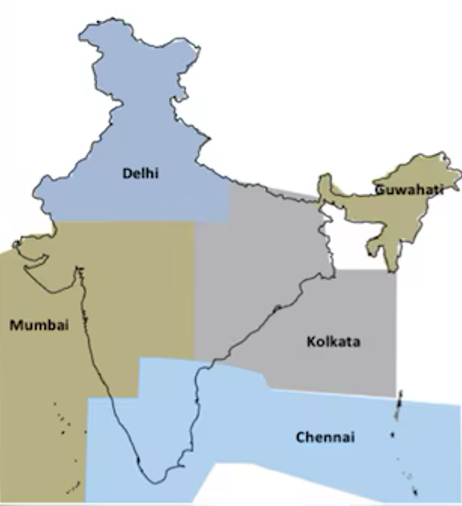
\includegraphics{img/indian-fir.png}
%     \caption{Current Indian airspace \glspl{FIR} \cite{chopra2024atm}.}
%     \label{fig:indian-fir}
% \end{figure}



% \subsection{Upgrades on ATC Infrastructure and ATCO Trainings}


% \subsection{Transition to Satalite Systems}

% Ground-based \gls{ATM} is the traditional system that uses infrastructure on the ground that supports the safe and efficient movement of aircrafts \cite{skybraryATM}.
% Examples include radar systems, flight control centers with \glspl{ATCO} and radio communications \cite{atmexcite2025satellite}.
% This system is often limited by geography and often struggles with tracking planes in areas outside its range \cite{atmexcite2025satellite}.

% The move towards a satalite \gls{ATC} brought about significant advancements in \gls{ATM} and offer real-time, global coverage of air traffic across the world's skies \cite{atmexcite2025satellite}.
% This advancement is particularly crucial as \gls{ATC} is no longer confied to specific regions like in the traditional system and offer a safer and more efficient \gls{ATM} in even the most congested or isolated airspace \cite{atmexcite2025satellite}.

% \gls{GPS} and \gls{GNSS} are examples of satallite-based systems that can significantly improve the accuracy of flight paths.
% Their integration to \gls{ATM} reduces errors caused by outdated or incomplete radar data, which can lead to miscommunication or unsafe distance separation between aircrafts \cite{atmexcite2025satellite}. 
% Aircrafts equipped with \gls{GPS} and \gls{GNSS} can safely navigate in regions previously deemed difficult to manage, such as remote or congested airspaces \cite{atmexcite2025satellite}. 
% As these systems provide accurate and real-time position information, these satellite systems help \glspl{ATCO} to make better informed decisions, ultimately reducing the likelihood of collisions \cite{atmexcite2025satellite}. 

% Legacy systems were not designed to support the precision and real-time data provided by satellite technologies, and calls for a need for significant infrastructure upgrades \cite{atmexcite2025satellite}. 
% This will be further explained in the next section.

\subsection{Infrastructure Upgrades}

As the legacy (or outdated) systems are not designed to support the precision and real-time data provided by satellite technologies, it calls infrastructure upgrades. 



% \subsection{Remote and Digital Tower Service}

% \gls{RTS} is a system which allows aerodrome \gls{ATC} or \gls{FIS} to be provided from a location other than the aerodrome (away from the physical airport tower) whilst maintaining a level of operational safety which is equivalent to that achievle using a manned Tower at the aerodrome to oversee both air and ground movements \cite{skybrary_rts}. 
% Its first opperational approval in the world was granted to Swedisch ANSP Luftfartsverket by the Swedisch Transport Agency in October 2014.
% Since then, only several countries and regions have embrached \gls{RTS} \cite{globalaero2024remote}, 

% An example would be the \gls{ATC} for London City Airport (LCY) is performed in NATS's air traffic control centre in Swanwick, Hamsphire, approximately 108 miles (173 km) away from LCY, with operations commenced in 2021 \cite{lcy2022digital}. 
% At LCY, \gls{ATC} is provided by a digital system, which sees 14 high-definition cameras and sensors mounted ona landside mast at the airport, which provide a 360 \textdegree view of the airfield \cite{lcy2022digital}. 

% An RTS combines advanced technology, real-time visual feeds and efficient communication to enhance air traffic control while allowing controllers to operate remotely.
% An RTS requires a number of high-definition cameras/sensors along with a vast network of signal cabling equipment to allow for fast data transfer (without lag) ensuring seamless communication between the controller and the aerodrome.

% \gls{RTS} is employed for the following reasons:
% \begin{itemize}
%     \item Cost savings: Building a remote tower typically requires a smaller unoccupied structure to house the cameras and equipment, whereas a conventional tower requires substantially more space. This means the construction costs are far lower for a remote ATC. Additionally, the maintenance costs on a conventional tower are higher due to the physical windows, radar screens and other specialised equipment.
%     \item Enhanced technology. Due to advancements in technology, air traffic controllers can observe aircraft through poor visibility or at night using infrared or high-definition cameras, or they can also use the enhanced zoom function to potentially spot wildlife on the runway that might not be visible with the naked eye. The remote ATC has advanced even further, providing an array of screens with detailed data such as runway conditions and other critical information. This data is fed into the livestream, meaning the controller doesn’t need to switch views constantly.
%     \item Staffing. Remote ATC towers are based at one location, which means controllers are no longer present at each airport. For aerodromes that have infrequent usage, you could use one controller to manage multiple aerodromes. This consolidation minimizes staff requirements, which results in cost savings. Given that controllers no longer need to work in a remote environment, there is a better work-life balance, which results in better workforce morale.
%     \item Safety Improvements. High-definition cameras and infrared technology give controllers better visibility, especially in nighttime operations. This assists with the monitoring of potential hazards. Additionally, through the integration of tracking technology, various sensors can offer multiple viewing angles, improving situational awareness.
% \end{itemize}




\subsection{Unifying Airspaces}




\subsection{UAS Traffic Management}





% \paragraph{Case Study:} \gls{NextGen} \cite{skybrary_nextgen}

\gls{NextGen} superceeds the \gls{NAS} of the United States, representing the evolution from a ground-based system of \gls{ATC} to satalite-based system of \gls{ATM}.
The combination of satallite-based and digital technologies and new procedures make air travel more convenient, predictable and environmental friendly in the US's increasing congested airspace.

It consists of five elements:
\begin{enumerate}
    \item \gls{ADS-B}: uses \gls{GPS} satellite signals to provide \glspl{ATCO} and pilots with much more accurate information that will keep aircraft safely separated in the sky and on runways.
    \item \gls{NDC}: using data communications to provide additional means of two-way communication, on top of the current voice communications between aircrew, \gls{ATC}, and \glspl{ATCO}.
    \item \gls{NNEW}: a single national weather information system that is updated in real time to provide a common weather picture across \gls{NAS}, and enable better air transportation decision making
    \item \gls{SWIM}: a single infrastructure and information management system to deliver data to many users, while also reducing the number and types of interfaces and systems, and reducing data redundancy
    \item \gls{NVS}: a single air/ground and ground/ground voice communications systemm, superceeding the current 17 different voice switching systems in the \gls{NAS}
\end{enumerate}

Through these elements, \gls{NextGen} assists with trajectory based operations of aircrafts and reducing any weather impacts in real time, providing pilots and \glspl{ATCO} with the same precise information transmitted via data communications, improving decision-making.
It also helps with the development of new procedures to improve the management of airports and terminals, increase the throughput to fly aircrafts in and out of many airports, especially high density airports.

% \paragraph{Case Study:} \gls{SESAR} Project \cite{ec_sesar_project} \cite{skybrary_sesar}

The \gls{SESAR} project is the \gls{EU}'s initiative aiming to modernise Europe's air and ground ATM infrastructure and operational procedures.
It is a joint effort driven by the \gls{EU}, EUROCONTROL, and a wide range of public and private, civil and military avaiation stakeholders to achieve the Digital European Sky.

The Digital European Sky leverages the latest technologies to transform Europe's aviation infrastructure, enabling it to handle the future growth and diversity of air traffic safely and effeciently, while minimising environmental impact.
It can increase the level of automation, cyber-secure data sharring and connectivity in \gls{ATM}, and virtualisation of its infrastructure and air traffic service provision in all types of airspaces (including very low and high-altitude operations).

It was identified in 2005 as a project of interest and its implementation is carried out in three phases:
\begin{enumerate}
    \item Definition phase (2005-2008): development of air traffic modernisation plan, establishing the different technological stages, priorities and timetables
    \item Development phase (2008-2013): development of basic technologies which will underpin the new generations of systems
    \item Deployment phases (2014-2020, and beyond): large-scale installation of the new systems and the widespread implementation of the related functions
\end{enumerate}





% \subsection{Upgrades on ATC Infrastructure}

% \subsubsection{Automation}


% \subsubsection{Training of ATCOs}



% \subsection{Unifying of Air Traffic Management}



% \paragraph{Case Study:} individual



% \subsection{Transition to ground-base to satalite systems}



% \subsection{Remote and Digital Towers}


% \subsubsection{Multi-Airport Coordination}



% \subsection{UAS Traffic Management}

% \subsubsection{Autonomous UTM}